%File: formatting-instruction.tex
\documentclass[letterpaper]{article}
\usepackage{aaai}
\usepackage{times}
\usepackage{helvet}
\usepackage{courier}
\usepackage{graphicx}
\usepackage{hyperref}
\frenchspacing
\setlength{\pdfpagewidth}{8.5in}
\setlength{\pdfpageheight}{11in}
\title{ A comparison between Restraining Bolts and Shielding \\ for Safe Reinforcement Learning}
\author{
   Robbe Louage\textsuperscript{1}, Elias Storme\textsuperscript{2}
   \\ 1 \texttt{robbe.louage@student.kuleuven.be}
   \\ 2 \texttt{elias.storme@student.kuleuven.be}
}
\pdfinfo{
/Title A comparison between Restraining Bolts and Shielding for Safe Reinforcement Learning
/Author Robbe Louage, Elias Storme}
\setcounter{secnumdepth}{0}  
 \begin{document}
% The file aaai.sty is the style file for AAAI Press 
% proceedings, working notes, and technical reports.
%
\maketitle
\begin{abstract} % Elias
\begin{quote}
Many approaches exist make a reinforcement learner behave in safer ways. This paper compares the performance of the restraining bolts and shielding methods. This is done using two board games: Sapientino and a Minecraft-like game. Sapientino does not really differentiate performance well between the approaches, due to its relatively low complexity. Minecraft shows much quicker convergence for shielding, with both agents achieving a comparable level of performance after 10000 episodes.
\end{quote}
\end{abstract}

\section{Introduction} % Elias
Enforcing safe behavior onto reinforcement learners has recently become a hot topic in AI research. Making sure an agent follows a safety specification is of course desirable in a variety of situations, especially when the agent is to be deployed into the real world. 
Many approaches have been proposed in literature. In this report, we will compare the performance of two of these techniques: restraining bolts \cite{de2019foundations} and shielding \cite{alshiekh2018safe}.
\par For completeness, this introduction will give a short overview of the concepts which were discussed at length during the presentation and in the papers. The techniques we are comparing have a lot in common when it comes to the environment they operate in. They both deal with safe reinforcement learning within a Markov decision process. Game theoretically this means we are doing reinforcement learning in a single agent environment on a stochastic game.
\par Restraining bolts is a technique which takes inspiration from science fiction. In the film Star Wars at one point the droid protagonists are fitted with restraining bolts, making it seemingly "painful" for the droid to perform certain actions which are deemed undesirable. This translates quite well into the realm of RL when we give the agent negative rewards for bad behavior. More concretely the restraining bolt becomes an automaton which observes the environment alongside and independently from the agent, observes the action taken by the agent, and finally gives the agent an appropriate reward.
\par Shielding takes a more drastic approach than RB, taking a position in between the agent and the environment and having the ability to intercept and change bad behavior. In practice this translates into a very similar setup. The shield also takes the form of an automaton, observing the world alongside and independent from the learner. However, this time the agent submits its action to the shield, which then decides based on its state what action to take and to submit to the environment. The shield does not however give rewards to the agent.
\\ \par In the following sections we will compare the performance of these two approaches to enforcing safe agent behavior. We will mainly focus on their impact on convergence, selecting some other metrics where deemed relevant. Alongside this comparison we will include the details which got lost during the presentation. Methodology and tuning of variables will be discussed as they are relevant to how we obtained the results we obtained.

\section{Sapientino} % Elias
Sapientino is a children's board game. An implementation of this game in pygame was included with the paper, its abstraction of the game board is shown in figure \ref{fig:sapientino}. The objective of the game is to match concepts. These matching concepts are represented here by squares of the same color. The player moves around the board and puts "bips" on squares. When the player consecutively bips two or more squares of the same color, those squares are matched and the player receives points. The actual implementation deviates from this reward system in a way we shall discuss later.
\begin{figure}[ht]
    \centering
    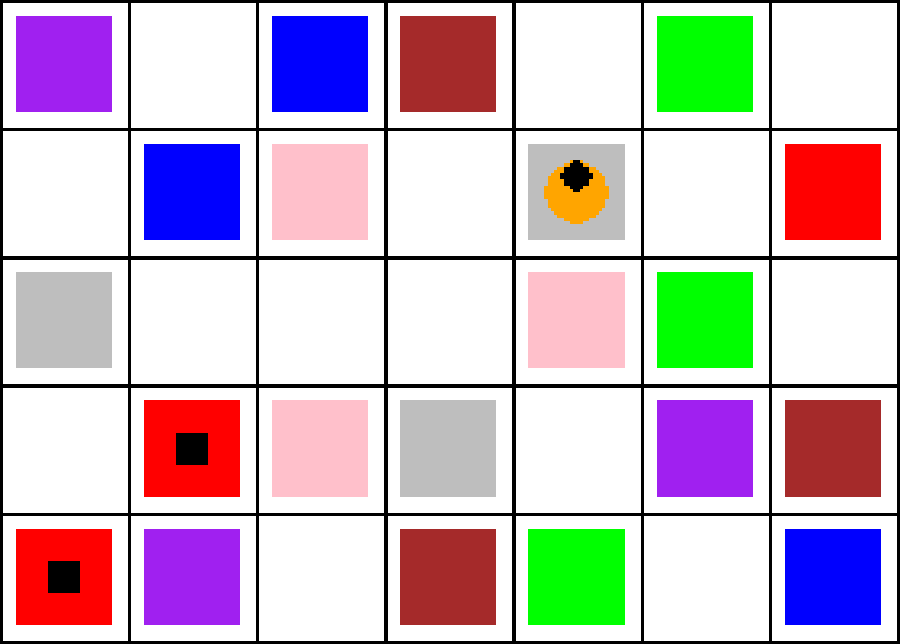
\includegraphics[width=.35\textwidth]{figs/sapientino.png}
    \caption{Sapientino game board}
    \label{fig:sapientino}
\end{figure}
\par This game was chosen because of its simplicity in implementation and safety specification. The safety specification imposed by the authors is that all 3 squares of a color have to be bipped consecutively, as well as an order in which the colors have to be bipped: red, green, blue, pink, brown, gray, purple. The reward structure for this game, as implemented is the following. Each time the agent places a correct bip, it earns 100 reward points. Completing the game yields 1000 points. Putting a bip on a wrong color, or an uncolored square yields -10 points and ends the game.

\subsection{Shield implementation}
As the safety specification gets broken by one action, this makes the implementation of a shield automaton quite straightforward. In sapientino our approach was to let the agent take an action an "simulate" what its effect is on the environment. The agent chooses an action and submits it to the environment. The reward automaton, originally implemented for the restraining bolt then checks if the state reached by executing the chosen action violates the safety specification. If this is the case, the environment and reward automaton states are reverted to their original state, and another action is chosen at random. Remark putting a bip on an empty square does not violate the safety specification. As such, we do not revert state in that case and just let the episode terminate.
\par In hindsight, using a random action may not have been the best approach. Better would have been to let the agent rank its actions based on utility. The original implementation of the learner didn't allow for this easily however. For this reason, we originally opted not to incorporate this. As we will discuss later, for the minecraft implementation we did add this feature.
\subsection{Methodology}
For testing we selected three metrics: cumulative reward during learning, final policy reward and final policy number of actions. In order to prevent the agent from getting stuck in local minima during learning, and to smooth the data to make it more legible, 50 runs of learning were done. We explain in more detail how the data for each metric was collected. 
\par The parameters for the learning agent were as follows. We took a discount factor $\gamma = .9$, which was the value suggested by the authors. For greedyness we set $\epsilon = -2$, which obviously isn't a real value for the regular epsilon-greedy action selection mechanism. The values -2 and -1 engage the adaptive modes, of which -2 worked best for us. The Q update was set to update 10 actions in the past, which again was a value suggested by the authors. 
\par During a learning run, we let the agent learn for 1000 episodes of the game. For each episode, the earned reward was recorded. The mean of this reward was then taken per episode, producing the plot in figure \ref{fig:learning_reward}. 
\begin{figure}[ht]
    \centering
    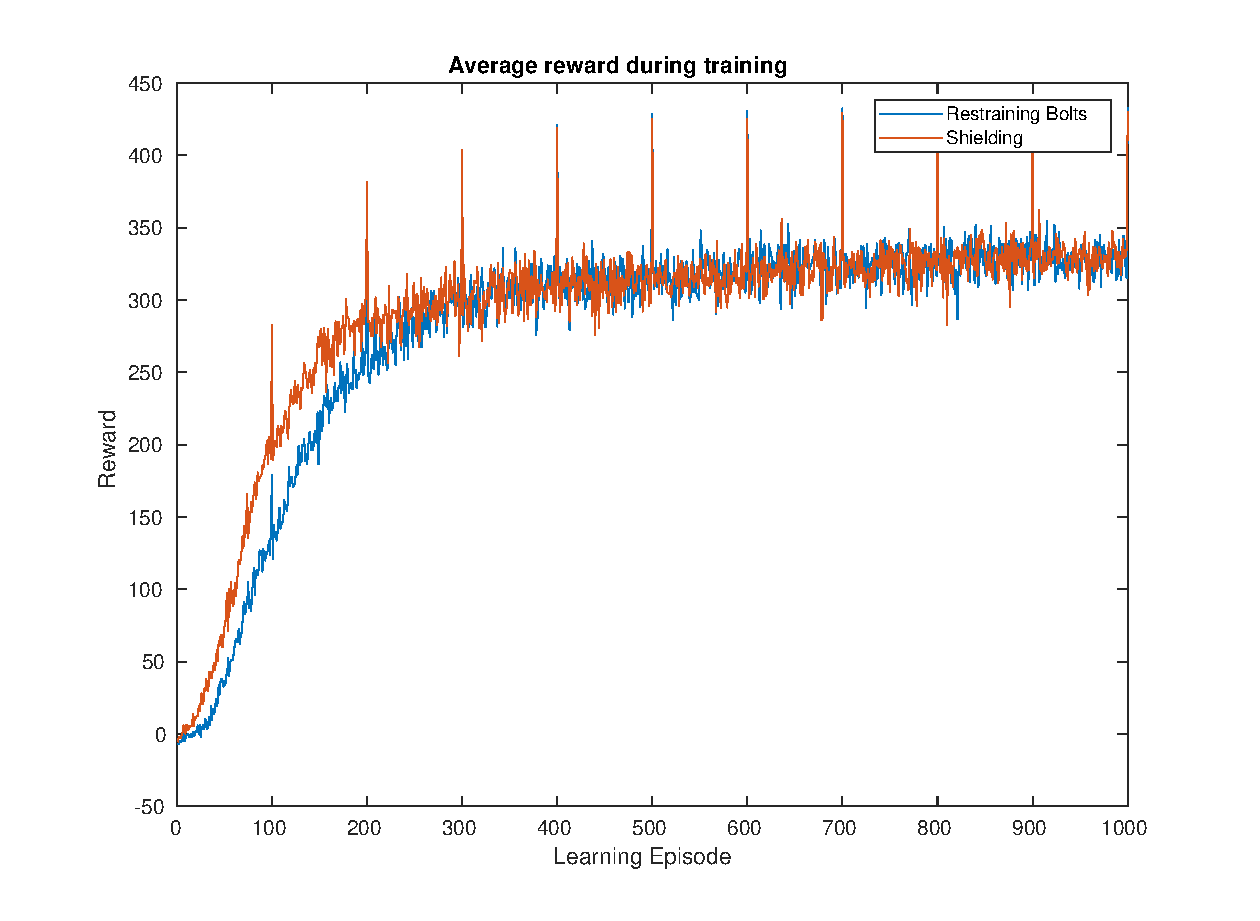
\includegraphics[width=.5\textwidth]{figs/sapientino_learning_reward.eps}
    \caption{Sapientino: reward during learning}
    \label{fig:learning_reward}
\end{figure}
\par In the plot we see weird peaks suspiciously located at every 100th episode. As we have written a custom script to produce these results, that was the first thing we looked at for a possible explanation. It is possible we used the wrong variable to get the reward per episode, as is always a risk when building upon another person's code. To mitigate this we turned to the original \texttt{game.py} script included in the paper. This trains the agent on a given game, and records a whole battery of different metrics including the reward per episode. We ran 12 samples of this, and combined the results of each of the different runs in the same way in MATLAB, by taking the mean of the rewards grouped per episode. This produced the plot in figure \ref{fig:sapientino_game_py}. 
\begin{figure}[h]
    \centering
    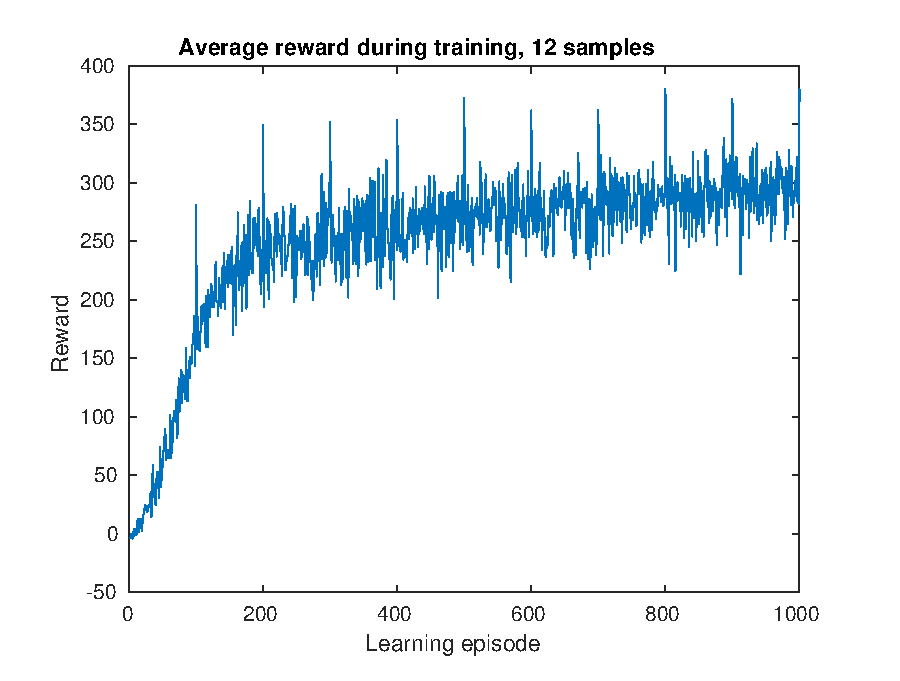
\includegraphics[width=.5\textwidth]{figs/sapientino_reward_game_py.eps}
    \caption{Sapientino: rewards recorded by \texttt{game.py}}
    \label{fig:sapientino_game_py}
\end{figure}
\par We see the same kind of spikes as earlier, indicating the problem does not originate within our code. The only transformation we applied was averaging within episodes, so that should not affect the results. There must be some bug within the code that generates these spikes. It is however not detectable within the data of a single training run, as the reward data is very noisy and spiky unless you do averaging like we did.
\par We decided not to dig any deeper into this for two reasons. Firstly because the spikes every 100 episodes do not obscure any trends which we might observe. Secondly, we have additional metrics with which we can confirm observed behavior such as the episode score. This led us to conclude that time which we could spend investigating what bug was causing this, would be better spent implementing shielding on another game.
\par After 1000 learning episodes, the policy is evaluated for 10 runs. During this evaluation, the agent does not update its Q values, and turns off the epsilon-greedy action selection mechanism. In other words, it gets put into pure exploitation mode. In evaluation we were interested in the reward the agent achieves, and the number of actions it takes during an episode. This time we take the mean of the rewards and the number of actions per final policy. 
\begin{figure}
    \centering
    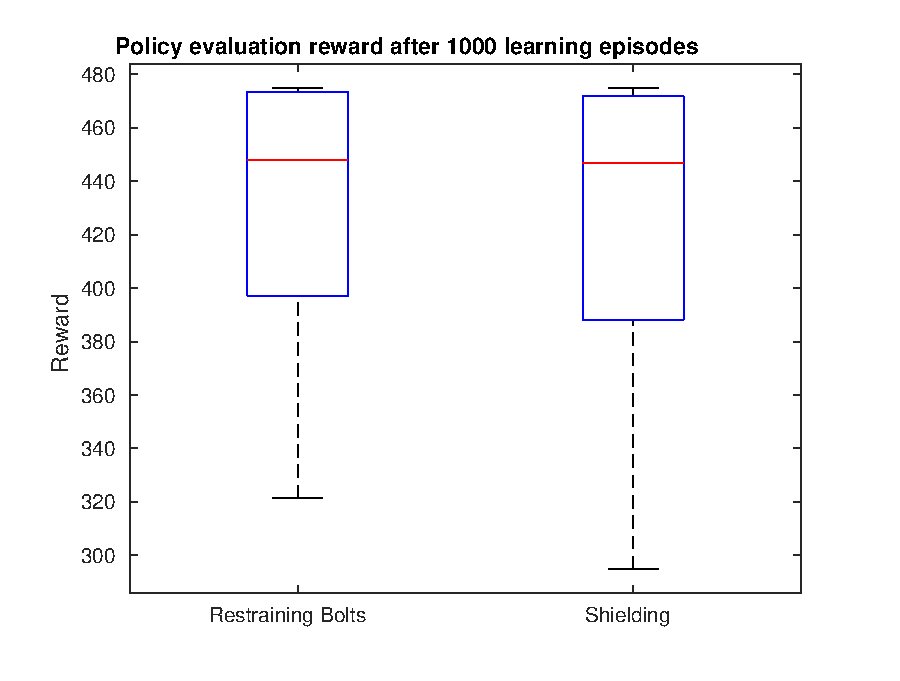
\includegraphics[width=.5\textwidth]{figs/policy_reward.eps}
    \caption{Sapientino: final policy rewards}
    \label{fig:sapientino_policy_reward}
\end{figure}
\subsection{Results}
During training, we see slightly faster convergence for the agent using shielding. Both agents however converge sufficiently quickly to a policy which almost always wins the game. This is reflected in the boxplot for the reward during policy evaluation. The resulting policies achieve on average the same reward during an episode. Looking at the number of actions resulting from the policy, we see a little differentiation. On average the number of actions is the same, but the interquartile range is slightly larger for shielding. This suggests the policy resulting from learning with shielding has a higher probability to take more actions than a policy learned using restraining bolts.
\begin{figure}
    \centering
    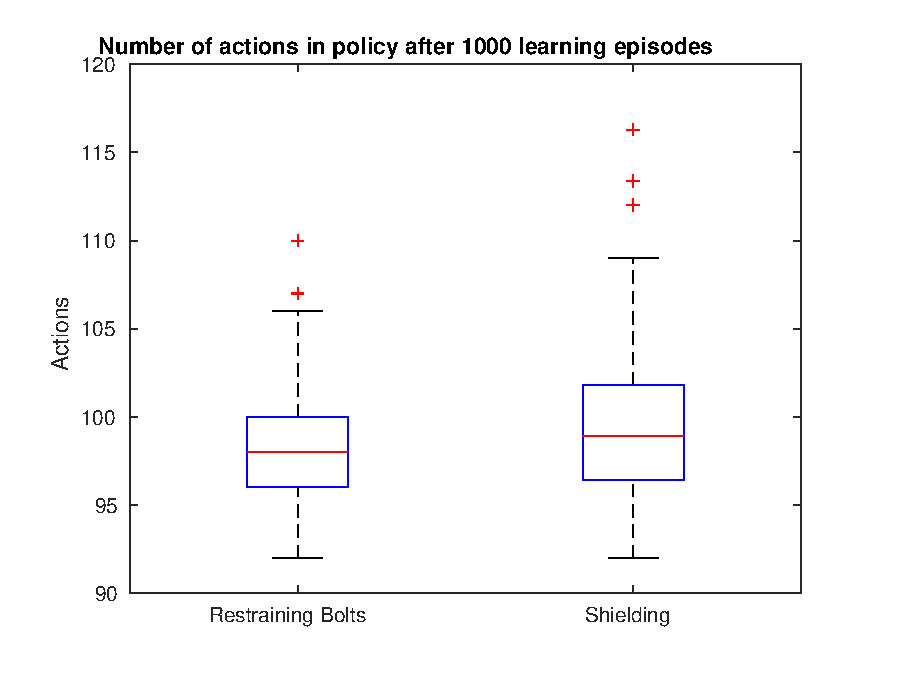
\includegraphics[width=.5\textwidth]{figs/policy_actions.eps}
    \caption{Sapientino: final policy no. of actions}
    \label{fig:sapientino_policy_actions}
\end{figure}
\par All things considered, the results from comparing the approaches on the game sapientino are not conclusive. This was also the feedback given during the presentation. The hypothesised reason for this inconclusiveness was the relative lack of complexity of the game. Knowing this, we decided to implement shielding on another, more complex game, which is discussed in the next section.
\section{Minecraft} % Robbe
The second game we chose to test the two approaches was a Minecraft like game, for which the environment is shown in figure \ref{fig:minecraft} (Minecraft concept used from Icarte et al. 2018). 
In this game the agent has to complete
some tasks in no particular order. For each task the agent has to get some items and use them
or make more advanced items in a work space. Each color represents an item or a work space. For example one of tasks is to make a gem. The agent has to get wood, use it on a workbench, get iron, use the tool shed and use the axe on the made item. 
\par This game is much more complex than Sapientino. Here the agent has to accomplish 10 tasks (described
with non-Markovian rewards via an $LTL_f$ / $LDL_f$ formula).
The agents gets one point per task it completes.
The same agent from Sapientino is used.
This game was chosen because it resolves some of the problems we had with the previous game. First of all the agent doesn't stop an episode when it is in a \textit{bad} state. In Sapientino the agent was in a bad state when it placed a bip on the wrong color. In Minecraft the agent is in a bad state when it uses an item or work place when it doesn't have to. An average episode is also much longer than in Sapientino, around 150-300 actions are performed. In our configuration the Minecraft environment had 10 rows and 10 colomuns. 
\par We first trained the bolts agent with the Q-learning algorithm with an adaptive greedy factor and a discount factor $\gamma$ of 0.9 on the game. Then we implemented a shield for this game and let the agent train with the same parameters. The shield prevents the agent to get in bad states. 
An episode ends when the agents has performed a certain number of actions or when the agents did get in too many bad states. Because the agents doesn't get in bad states with shields the episodes tend to be longer. To compensate for this difference we shortened the maximum number of actions before an episode ends. With the shortened episodes the shield agent didn't seem to find good policies so we increased the maximum number of actions and the shield agent performed much better. If the shield agent would get in a bad state
the agents performs the second-best action it could perform that would not result in a bad state. The reward from this action is given.
\begin{figure}
    \centering
    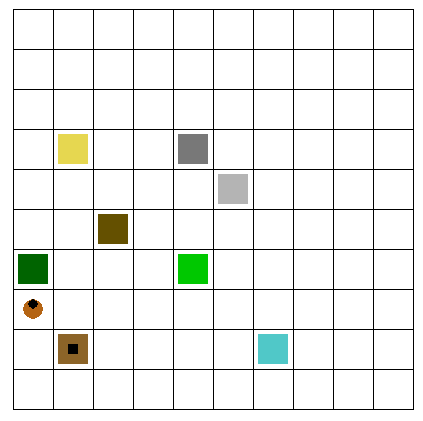
\includegraphics[scale=0.5]{figs/minecraft.png}
    \caption{The Minecraft like environment}
    \label{fig:minecraft}
\end{figure}
\subsection{Results}
In the following two figures (\ref{fig:minecraftScore}, \ref{fig:minecraftReward}) we plot the moving average from the last 100 episodes for both agents for both the score and the reward.
\begin{figure}[ht]
    \centering
    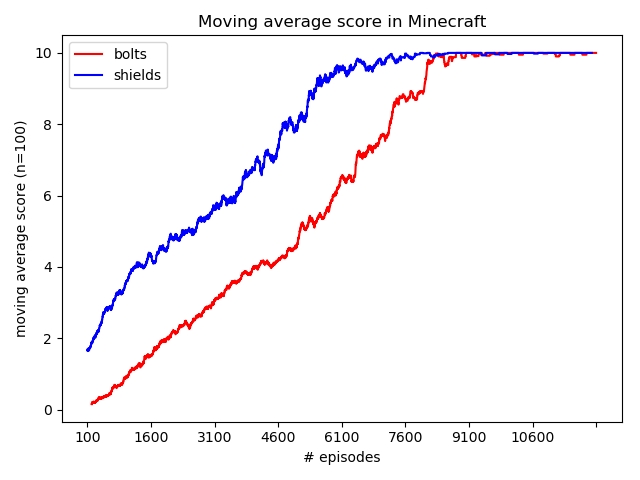
\includegraphics[scale=0.35]{figs/score_boltz_shields_Minecraft.png}
    \caption{The moving average score for both agents on the Minecraft like game}
    \label{fig:minecraftScore}
\end{figure}
\begin{figure}[ht]
    \centering
    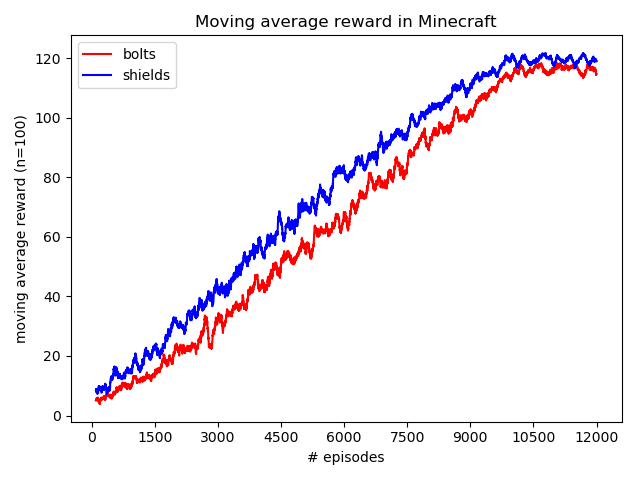
\includegraphics[scale=0.35]{figs/reward_boltz_shield_minecraft.png}
    \caption{The moving average reward for both agents on the Minecraft like game}
    \label{fig:minecraftReward}
\end{figure}
We clearly see that the shielding agent performs much better in the episodes before reaching the maximum score. The same results can be observed from the reward plot. We however don't see a faster significant faster convergence rate to an optimal policy. A important observation is that both agents arive at different policies. The shielding agent performs the maximum score in 177 actions and the bolts agents in 200 actions. This difference is possibly explained by the fact that there is no specification given on how long the total path can be, only the tasks are relevant. 

\section{Discussion} % Robbe
In the shields paper the authors see a great improvement in the performance of the learner in all their experiments. We however only see this effect partially. In the Sapientino game the improvement can possibly be explained because the search space is limited and the shielding agent has less of a chance to perform an wrong action. In the Minecraft game this probably is not the reason because the search space is much larger and much more complex. We do however see a clear improvement in the performance in the early and middle episodes.  \\
In an ideal world, we would test both agents much more and on more games. But because of the difficulty to interact with both code bases this was a hard task. Also writing a safety specification for a game is a difficult task with which we had no experience. \\
Another downside for a shield agent is that it has to \textit{simulate} the action which it will perform to check whether it will result in a bad state. this simulation can result in a lot of overhead. If this is not well implemented this can double the running time of learning process.

\section{Running paper code} % Elias
As part of the preparation for both the presentation and the creative part, quite some time was spent trying to run the code included in both papers. This was done for several reasons. Firstly, it provides excellent insight in how the authors of the paper intended their ideas to be implemented. This allows us to in turn understand the papers better. Additionally, we used the code as a starting point for our creative part, and ended up reusing a lot of the code included with the restraining bolts paper.
\par The reason we gravitated towards the RB code, was our difficulty in running the code included with the shielding paper. Documentation was quite poor, especially with the shield generation tool as discussed by the other group which was assigned this paper. Additionally, there were issues with the dependencies. The included dependency list was for a weird combination of outdated packages, which were difficult to get installed on our systems at all. Deviating from the exact versions specified yielded some strange errors indicating the code was using some packages in an inappropriate way. An example of such an outdated package is Tensorflow 1.3, which dates from august 2017. The paper includes some claims on training speed on a GPU using tensorflow. We would have loved to confirm these results, and gave it a shot. The code was not compatible with the 1.15 release of tensorflow, and getting the right combination of drivers installed to run tensorflow 1.3 with CUDA on a modern system proved very difficult. We decided this was not worth the time. In hindsight, docker may have been a viable way to obtain the right runtime environment. At the time however, we were not experienced enough with that software to quickly put something together.

\section{Course evaluation} % Robbe
This course was a different kind of course. We both didn't really experience this kind of freedom to implement our own idea. During the course we probably should have contacted the assistants much more. Sometimes we could get stuck on some part
and didn't really have a clear solution. During the last presentations we learned a lot and should've spent our time more efficiently. \\
The communication of this course were somtimes a bit lacking. The group wiki on Toledo wasn't always very clear.
We both liked that this course focuses on new research and had a lot of fun to read and play with the latest findings in reinforcement learning. We now also have a more clear understanding of what safety means in the context of reinforcement learning. \\
In total we spent about 20 hours reading research papers and doing general research. About 50 hours understanding and implementing the paper code and our experiments and about 10 hours writing the reports. All these numbers are per person. This puts our time spent slightly above the time provisioned by the study points, but not dramatically so.


\section{Conclusion}% Robbe
We tested a restraining bolts agent and a shields agent on two games: Sapientino and a Minecraft like game. In the first game the results were slightly promising, but not really conclusive. This may be explained by the relative lack of complexity in the game.
In the second much more complex game we still saw an improvement with the shields agent. These differences were harder to explain. The two agents have both their place in reinforcement learning and can be applied to different kind of problems. More research and tests are needed on much more complex games to have more decisive results. 


%\section{References} % elias
\nocite{*}
\bibliographystyle{aaai}
\bibliography{bibliography}

\end{document}